\documentclass{article}

\usepackage[left=2cm,right=2cm,top=2cm,bottom=2cm]{geometry} 

\usepackage[utf8]{inputenc}   % otra alternativa para los caracteres acentuados y la "ñ"
\usepackage[           spanish % para poder usar el español
                      ,es-tabla % para los captions de las tablas
                       ]{babel}   
\decimalpoint %para usar el punto decimal en vez de coma para los números con decimales

%\usepackage{beton}
%\usepackage[T1]{fontenc}

\usepackage{parskip}
\usepackage{xcolor}

\usepackage{booktabs,longtable,array}
\newcolumntype{L}[1]{>{\raggedright\let\newline\\\arraybackslash\hspace{0pt}}m{#1}}
\newcolumntype{C}[1]{>{\centering\let\newline\\\arraybackslash\hspace{0pt}}m{#1}}
\newcolumntype{R}[1]{>{\raggedleft\let\newline\\\arraybackslash\hspace{0pt}}m{#1}}

\usepackage{caption}

\usepackage{enumerate} % paquete para poder personalizar fácilmente la apariencia de las listas enumerativas

\usepackage{graphicx} % figuras
\usepackage{subfigure} % subfiguras

\usepackage{amsfonts}
\usepackage{amsmath}

\usepackage{colortbl}

\usepackage{listings}
\lstset
{ %Formatting for code in appendix
    language=python,
    basicstyle=\footnotesize,
    stepnumber=1,
    showstringspaces=false,
    tabsize=1,
    breaklines=true,
    breakatwhitespace=false,
}

\definecolor{softpink}{rgb}{1,0.8,1}
	
\usepackage{float} % para controlar la situación de los entornos flotantes

\restylefloat{figure}
\restylefloat{table} 
\setlength{\parindent}{0mm}


\usepackage[bookmarks=true,
            bookmarksnumbered=false, % true means bookmarks in 
                                     % left window are numbered
            bookmarksopen=false,     % true means only level 1
                                     % are displayed.
            colorlinks=true,
            allcolors=blue,
            urlcolor=blue]{hyperref}
\definecolor{webblue}{rgb}{0, 0, 0.5}  % less intense blue

\renewcommand{\thesection}{\arabic{section}}

\title{\Huge Inteligencia de Negocio: Práctica 3 \\ Competición de Kaggle\vspace{10mm}}

\author{\huge David Cabezas Berrido \vspace{10mm} \\ 
  \huge Grupo 2: Viernes \vspace{10mm} \\ \huge dxabezas@correo.ugr.es \vspace{10mm}}

\begin{document}
\maketitle

\pagebreak

\begin{figure}[H]
  \centering
  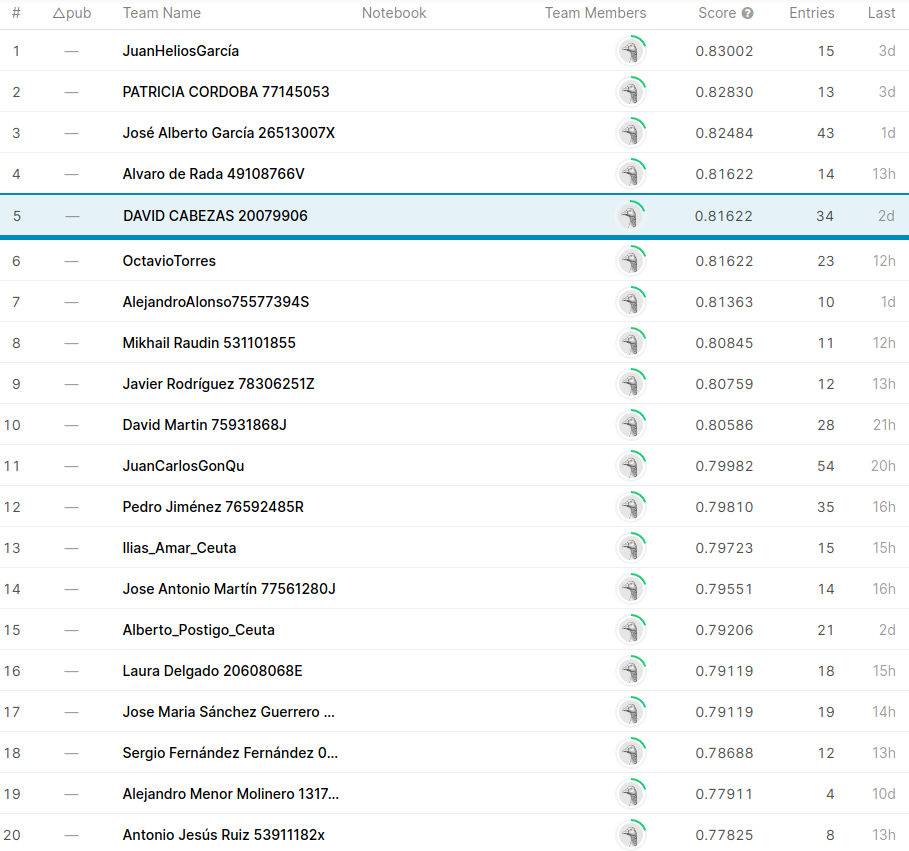
\includegraphics[width=180mm]{imgs/leaderboard}
  \caption{Leaderboard definitiva de la competición.}
  \label{fig:leaderboard}
\end{figure}

\pagebreak

\tableofcontents

\pagebreak

\section{Pruebas realizadas}
\setlength\LTleft{-0.5in}
\setlength\LTright{-2in}
\begin{longtable}{|c|C{2.1cm}|c|c|c|C{4cm}|C{6cm}|}
\toprule
Intento & Fecha-hora & Posición & Validación & Test & Preprocesado & Modelo \\

\midrule

1 & 19/12/2020 14:35:08 & 5 & 0.8185 & 0.7420 & Preprocesado 1 & RandomForest por defecto \\

\arrayrulecolor{black!10}\midrule

2 & 20/12/2020 10:51:19 & 4-5 & 0.8900 & 0.7580 & Preprocesado 2 & RandomForest por defecto \\

\arrayrulecolor{black!10}\midrule

3 & 20/12/2020 12:34:18 & 4-5 & 0.9040 & 0.7498 & Preprocesado 2 eliminando de train los ejemplos que inicialmente tenían descuento & RandomForest con 350 estimadores de profundidad máxima 20 \\

\arrayrulecolor{black!10}\midrule

4 & 20/12/2020 17:05:16 & 3-4 & 0.9179 & 0.7645 & Preprocesado 3 & MLPClassifier con capas ocultas de tamaño (200,200) \\

\arrayrulecolor{black!10}\midrule

5 & 21/12/2020 09:47:11 & 3-4 & 0.8750 & 0.6877 & Preprocesado 3 & 2-NN con distancia Manhattan y pesos inversamente proporcionales a la distancia \\

\arrayrulecolor{black!10}\midrule

6 & 21/12/2020 13:30:36 & 3 & 0.9143 & 0.7739 & Preprocesado 3 & C-SVM con C=65 y kernel RBF \\

\arrayrulecolor{black!10}\midrule

7 & 21/12/2020 15:32:20 & 3 & 0.9144 & 0.7645 & Preprocesado 3 & RandomForest por defecto \\

\arrayrulecolor{black!10}\midrule

8 & 22/12/2020 09:49:44 & 2 & 0.9143 & 0.8059 & Preprocesado 3 & GradientBoosting con 500 estimadores \\

\arrayrulecolor{black!10}\midrule

9 & 22/12/2020 09:50:03 & 2 & 0.9304 & 0.8016 & Preprocesado 3 & Stacking: - RandomForest por defecto - MLPClassifier con capas ocultas (200,200) - C-SVM con C=65 y kernel RBF - GradientBoosting con 500 estimadores \\

\arrayrulecolor{black!10}\midrule

10 & 22/12/2020 14:40:39 & 2 & 0.9312 & 0.7636 & Preprocesado 3 & AdaBoost con 500 árboles de profundidad 12 y learning rate de 1.1 \\

\arrayrulecolor{black!10}\midrule

11 & 23/12/2020 10:24:20 & 2 & 0.9163 & 0.7990 & Preprocesado 3 sustituyendo los valores perdidos por 0 en la columna descuento en lugar de eliminar la columna & GradientBoosting con 500 estimadores \\

\arrayrulecolor{black!10}\midrule

12 & 23/12/2020 12:12:38 & 2 &  & 0.7998 & Preprocesado 3 & Moda (predicción más frecuente) de los intentos 4, 6, 7, 8, 9, 10 y 11 \\

\arrayrulecolor{black!10}\midrule

13 & 24/12/2020 19:54:10 & 2 & 0.9205 & 0.7886 & Preprocesado 3 & GradientBoosting con 500 árboles de profundidad 6, learning rate de 1.175 y submuestras del 70\% \\

\arrayrulecolor{black!10}\midrule

14 & 25/12/2020 09:59:17 & 4 & 0.8535 & 0.7239 & Preprocesado 3 + PCA con 0.95 de varianza explicada & GradientBoosting con 500 estimadores \\

\arrayrulecolor{black!10}\midrule

15 & 25/12/2020 10:25:21 & 4 & 0.9159 & 0.8007 & Preprocesado 3 tras corregir error en LabelEncoder & GradientBoosting con 500 estimadores \\

\arrayrulecolor{black!10}\midrule

16 & 25/12/2020 11:33:44 & 4 &  & 0.8093 & Preprocesado 3 & Stacking de cuatro GradientBoosting con número de estimadores 450, 500, 550 y 600 respectivamente; tasas de aprendizaje 0.14, 0.12, 0.1, 0.08 respectivamente; todos con submuestras del 90\% \\

\arrayrulecolor{black!10}\midrule

17 & 26/12/2020 10:58:03 & 4 &  & 0.8085 & Preprocesado 3 & Stacking anterior con la opción passthrough \\

\arrayrulecolor{black!10}\midrule

18 & 26/12/2020 11:12:21 & 4 & 0.9268  & 0.7886 & Preprocesado 3 & HistGradientBoosting por defecto \\

\arrayrulecolor{black!10}\midrule

19 & 26/12/2020 11:31:13 & 4 & & 0.8024 & Preprocesado 3 & Stacking de tres
GradientBoosting con 500, 550 y 600 estimadores respectivamente; tasas
de aprendizaje 0.12, 0.1 y 0.08 respectivamente; todos con submuestras
del 90\%. También tres HistGradientBoosting con 100, 150 y 200 iteraciones máximas respectivamente \\

\arrayrulecolor{black!10}\midrule

20 & 27/12/2020 11:00:35 & 4 &  & 0.8016 & Preprocesado 3 & Stacking de cuatro GradientBoosting con número de estimadores 450, 500, 550 y 600 respectivamente; tasas de aprendizaje 0.14, 0.12, 0.1, 0.08 respectivamente; todos con submuestras del 90\%. También dos HistGradientBoosting con 100 y 200 iteraciones máximas respectivamente \\

\arrayrulecolor{black!10}\midrule

21 & 27/12/2020 13:54:7 & 4 & (0.8392) & 0.7886 & Preprocesado 3 & GradientBoosting con 550 árboles de profundidad 2, tasa de aprendizaje de 0.15 y submuestras del 90\% \\

\arrayrulecolor{black!10}\midrule

22 & 27/12/2020 14:30:41 & 4 & (0.8462) & 0.7790 & Preprocesado 3 & LightGBM con 125 árboles de profundidad máxima 8 y 27 nodos hoja como máximo; tasa de aprendizaje del 0.08 \\

\arrayrulecolor{black!10}\midrule

23 & 28/12/2020 09:21:46 & 4 & 0.9290 & 0.7808 & Preprocesado 3 & LightGBM con 200 árboles con profundiad máxima 14 \\

\arrayrulecolor{black!10}\midrule

24 & 28/12/2020 09:22:13 & 4 & 0.9291 & 0.7843 & Preprocesado 3 & LightGBM con 125 árboles con 29 nodos hoja como máximo; tasa de aprendizaje del 0.11 \\

\arrayrulecolor{black!10}\midrule

25 & 28/12/2020 09:16:14 & 4 & 0.9266 & 0.7817 & Preprocesado 3 & LightGBM por defecto \\

\arrayrulecolor{black!10}\midrule

26 & 29/12/2020 10:42:25 & 4 & \begin{tabular}[c]{c} (0.8151) \\ 0.8990  \end{tabular} & 0.7964 & Preprocesado 3 & MLP con early stopping \\

\arrayrulecolor{black!10}\midrule

27 & 29/12/2020 10:52:45 & 4 & \begin{tabular}[c]{c} (0.7920) \\ 0.9135  \end{tabular}  & 0.778 & Preprocesado 3 & SVM con C=40 \\

\arrayrulecolor{black!10}\midrule

28 & 29/12/2020 13:27:51 & 4 & \begin{tabular}[c]{c} (0.8352) \\ 0.9207 \end{tabular}  & 0.8016 & Preprocesado 3 & XGBoost con 200 árboles de profundidad 3 \\

\arrayrulecolor{black!10}\midrule

29 & 30/12/2020 09:45:53 & 4 & \begin{tabular}[c]{c} (0.8370) \\ 0.9262  \end{tabular}  & 0.7929 & Preprocesado 3 & HistGradientBoosting con 75 iteraciones máximas \\

\arrayrulecolor{black!10}\midrule

30 & 30/12/2020 09:43:11 & 4 & 0.9300  & 0.7774 & Preprocesado 3 & HistGradientBoosting con 200 iteraciones máximas, tasa de aprendizaje del 0.08 y árboles con 29 nodos hoja como máximo \\

\arrayrulecolor{black!10}\midrule

31 & 30/12/2020 10:08:35 & 4 & 0.9304  & 0.8110 & Preprocesado 3 & Stacking de GradientBoosting con 500 estimadores, MLP con early stopping, XGBoost con 200 árboles de profundidad 3 y HistGradientBoosting con 75 iteraciones máximas \\

\arrayrulecolor{black!10}\midrule

\rowcolor{softpink}

32 & 31/12/2020 10:14:38 & 5 & 0.9268  & 0.8162 & Preprocesado 3 & Stacking de GradientBoosting con 500 estimadores, MLP con early stopping y XGBoost con 200 árboles de profundidad 3 \\

\arrayrulecolor{black!10}\midrule

33 & 31/12/2020 11:29:18 & 5 & 0.9225  & 0.8067 & Preprocesado 3 & Stacking de GradientBoosting con 500 estimadores y y XGBoost con 200 árboles de profundidad 3 \\

\arrayrulecolor{black}\bottomrule
\caption{Pruebas realizadas}
\label{tab:pruebas}
\end{longtable}

\textbf{Nota:} Los valores entre paréntesis en la columna de
validación no corresponden a validación cruzada, sino a un conjunto de
validación que he separado para paliar un problema de sobreajuste. Ver Sección \ref{val-sobreajuste}.

\textbf{Nota 2:} El intento $n$, corresponde al archivo
\texttt{try$n$.csv}, pero en Kaggle corresponde al $n+1$ debido a que
subí un intento corrupto por un error en el formato de la salida.

\pagebreak

\section{Introducción}

Abordamos en una competición de Kaggle un problema del mundo real como
es la predicción del precio de un coche usado, o en este caso la
clasificación en categorías por precio. Probamos varias técnicas de
preprocesado y varias configuraciones de distintos modelos que hemos
estudiado en la asignatura. Realizamos diversos experimentos e
intentamos ir mejorando nuestro score sobre test hasta conseguir el
nuestro mejor resultado posible. Se trata claramente de un problema de
aprendizaje supervisado (clasificación), y aplicaremos las técnicas y
modelos propios de este tipo de tarea.

\section{Preprocesados}

El número de datos que presentaban valores perdidos en alguna de las
columnas era bastante bajo, del orden de pocos cientos entre los cerca
de 4800 datos, y no hay valores perdidos en los datos de test; es por
ello que desechamos las instancias con valores perdidos en alguna de
las columnas. Una excepción es la columna Descuento, en la que la gran
mayoría de las instancias carecen de valor, por esta razón tomamos la
decisión de desechar la columna. Hablaremos sobre ella más tarde.

Una vez tratado el problema de los valores perdidos, probamos distintas técnicas de preprocesado.

El \textbf{Preprocesado 1} es el mínimo para que os algoritmos puedan
ejecutarse. Codificamos las variables categóricas con
\texttt{LabelEncoder}, primero nos quedamos con la marca del coche, ya
que hay cerca de 2000 modelos y son demasiados para que los algoritmos
puedan aprovechar la información sólo con los algo más de 4000 datos
de entrenamiento de los que disponemos. Convertimos Consumo, Motor\_CC
y Potencia a numérica: por ejemplo, el string \texttt{23.4 kmpl} se
convierte en el flotante 23.4. También codificamos la mano como
numérica (del 1 al 4).

Con este procesamiento sólo hemos probado el intento 1, seguidamente
intentamos mejorarlo.

Las clases están desbalanceadas, hay una (3) con casi la mitad de las
instancias de entrenamiento y otras con cerca del 5\% de las
instancias. Para balancearlas he probado dos técnicas que se nos
explicaron en el seminario sobre balanceo. La primera ha sido
undersampling, y la deseché por obtener resultados bastante peores con
Random Forest por defecto que el preprocesado 1. La segunda ha sido
oversampling con \texttt{SMOTE}, que corresponde al
\textbf{Preprocesado 2}. Esta técnica si ha supuesto una mejora
significativa y he decidido mantenerla. Con este preprocesamiento,
sólo he probado los intentos 2 y 3, éste último con una modificación que comentaremos en la Sección \ref{descuento}.

El \textbf{Preprocesado 3} aplica técnicas que acostumbran a
beneficiar a modelos como KNN, SVM y redes neuronales. Estas técnicas
son la binarización de características nominales y la estandarización
de los datos (reescalarlos y desplazarlos para que tengan media 0 y
varianza 1). He mantenido este preprocesamiento por el resto de
experimentos, añadiendo pequeñas variaciones en el intento 11
(relativa a la columna Descuento) y en el intento 14, en el que he
combinado este preprocesamiento con PCA para el 95\% de variabilidad
explicada, pero resultados peores.

En el intento 15, he corregido un error en el código que enumeraba
incorrectamente los valores de la columna Mano (el 1 debe corresponder
a primera mano, el 2 a segunda, el 3 a tercera y el 4 a cuarta o
más). También he aprovechado para eliminar la única instancia de
entrenamiento correspondiente a un coche eléctrico, ya que el conjunto
de test no presenta instancias correspondientes a este tipo de
coches. Todos los intentos posteriores se realizan con la nueva
versión corregida de este preprocesamiento, aunque no parece que el
error tuviese poca relevancia (de hecho el intento 15 obtiene peor
score en test que el 8, correspondiente al mismo modelo sin el arreglo
en los datos).

\pagebreak

\section{Estimación de hiperparámetros}

Para ajustar los hiperparámetros de los modelos, recurrimos a la
función
\href{https://scikit-learn.org/stable/modules/generated/sklearn.model_selection.GridSearchCV.html}{\texttt{GridSearchCV}},
que realiza validación cruzada (usamos 3, 4 o 5 folds, según lo rápido
que se ejecuten los modelos) para cada combinación en una cuadrícula
de valores para los hiperparámetros. Por ejemplo, el siguiente código
realiza la búsqueda para los hiperparámetros de KNN.
\begin{lstlisting}
param_grid={'n_neighbors':[1,2,3,5,7],'weights':['uniform','distance'],
            'metric':['euclidean','manhattan']}
searcher = GridSearchCV(model, param_grid, n_jobs=4,verbose=15,cv=4)
search = searcher.fit(train,label)
\end{lstlisting}
En este caso, prueba $5\cdot 2\cdot 2=20$ combinaciones, y realiza 4
fits y validaciones para cada una. Podemos obtener los resultados como
un DataFrame y ordenarlos por score medio.

\begin{figure}[H]
  \centering
  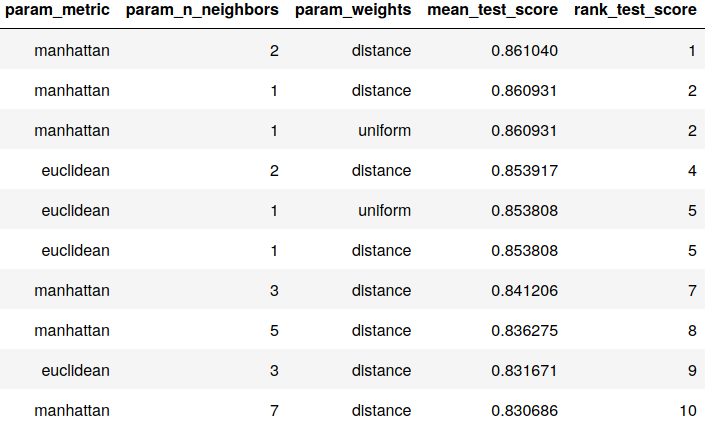
\includegraphics[width=140mm]{imgs/tune-knn}
  \caption{Score medio en CV para distintas configuraciones de KNN.}
  \label{fig:tune-knn}
\end{figure}

En ocasiones hemos realizado este proceso varias veces, detallando la
cuadrícula o ampliando el rango de valores de los parámetros cuyos
óptimos se encontraban en los extremos del rango.

\subsection{Sobreajuste con oversampling y validación
  cruzada} \label{val-sobreajuste}

Durante el desarrollo de la práctica, me he percatado de un problema
que provocaba sobreajuste en los modelos. Cuando generamos datos
sintéticos con \texttt{SMOTE} para el oversampling, obtenemos datos
muy similares a los datos originales. Por tanto, en el conjunto de
datos de entrenamiento hay instancias muy similares entre sí. Cuando
hacemos validación cruzada los algoritmos no entrenan con los mismos
datos con los que validan, pero si con datos muy similares, lo que los
lleva a sobreajustar. Esto provoca que las combinaciones de
hiperparámetros que obtienen mejores scores a la hora de validar sean
las que presentan bajo sesgo y alta varianza, por lo que no tienen que
tener un desempeño mejor sobre el conjunto de test. Según la teoría de
aprendizaje, la validación cruzada debería obtener una estimación
pesimista de la capacidad de generalización real del modelo. Con
scores de validación por encima de 0.9 y scores en test que apenas
alcanzan los 0.8, podemos sospechar que este problema está provocando
sobreajuste en los modelos y minando su desempeño sobre test en una
medida bastante significativa.

Para arreglar esto, separamos un conjunto de validación antes de hacer
oversampling, y evaluamos cada configuación de cada algoritmo sobre
este conjunto, de modo que los datos de validación no son tan
similares a los de entrenamiento y obtenemos validaciones más
realistas (rondando 0.8-0.84 de accuracy) y modelos con menos
varianza. Las configuraciones de los modelos cambian en gran
medida. GradientBoosting, que era mi mejor intento en ese momento, no
consigue superar su desempeño sobre test (los intentos 8 y 16 utilizan
árboles sin límite de profundidad, con este nuevo conjunto de
validación ajustamos los parámetros para el intento 21, que utiliza
árboles con profuncidad 2, pero obtiene peor score en test). En
cambio, los modelos SVM y MLP encuentran configuraciones con mayor
sesgo y menor varianza que logran superar a las anteriores
configuraciones. En el caso de SVM, pasamos de $C=65$ (intento 6) a
$C=40$ (intento 27), a menor $C$, mayor regularización, y conseguimos
una ligera mejora sobre el conjunto de test. Para MLP, obtenemos una
configuración más simple en la estructura de la red, de capas ocultas
con (200,200) en el intento 4 a (100) en el intento 26, además de la
incorporación de Early Stopping para regularizar, se consigue una
mejora bastante significativa sobre el conjunto de test. Introducimos
este último modelo en el Stacking correspondiente a nuestro mejor
intento (el 32).

\pagebreak

\section{Modelos}

Durante el desarrollo de la práctica probamos una amplia gama de
modelos de los que hemos estudiado en la asignatura.

\subsection{Random Forest}

Se trata de un modelo bastante robusto y adecuado para clasificación
multietiqueta. Trabaja relativamente bien con variables categóricos, y
no requiere que las variables presenten escalas similares, por lo que
no necesita un preprocesamiento tan complejo como otros modelos. Es
por ello que es el primer modelo que probamos para tener una idea de
los resultados que caben esperar. Se ve bastante beneficiado por el
balanceo de las clases (oversampling), y curiosamente también por la
binarización de características nominales (a pesar de trabajar bien
con categóricas) en el intento 7. No le hemos dedicado mucho más
trabajo a este modelo y no obtenemos buenos resultados con el ajuste
de hiperparámetros, probablemente por el sobreajuste que hemos
comentado antes. Los hiperparámetros que ajustamos son el número de
estimadores y la profundidad máxima de los mismos.

Para el resto de modelos, mantendremos la binarización de
características nominales y la estandarización de los datos, ya que
modelos como KNN, MLP y SVM requieren de estos preprocesados para
funcionar correctamente.

\subsection{MLP}

Los parámetros que ajustamos son la estructura de capas de neuronas
ocultas y el uso de Early Stopping para regularizar.

Obtiene resultados relativamente buenos en el intento 4 (los mejores
hasta el momento), sin Early Stopping y con una estructura compleja,
(200,200). Mejora mucho en el intento 26, cuando ajustamos parámetros
con el conjunto de validación y concluimos que es conveniente usar una estructura más simple, (100), y regularizar con Early Stopping.

\subsection{SVM}

Los parámetros que ajustamos son la regulariación $C$ y el kernel
usado. Rápidamente nos percatamos de que el kernel más efectivo es el
de Funciones de Base Radial (RBF), y tras varias búsquedas en grid,
elegimos el valor 65 para $C$.

\begin{figure}[H]
  \centering
  \subfigure[En la primera búsqueda nos decantamos por el núcleo RBF.]{
    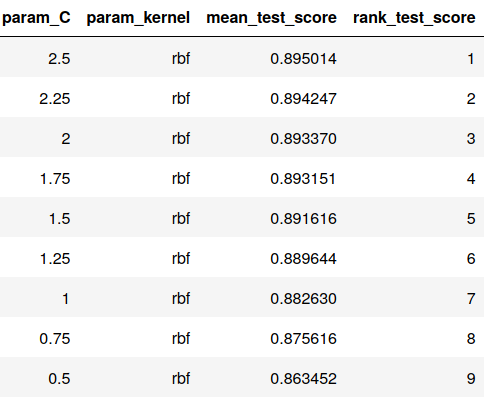
\includegraphics[width=55mm]{imgs/tune-svm1}
  }
  \subfigure[Los valores altos de $C$ consiguen mejor score en CV.]{
    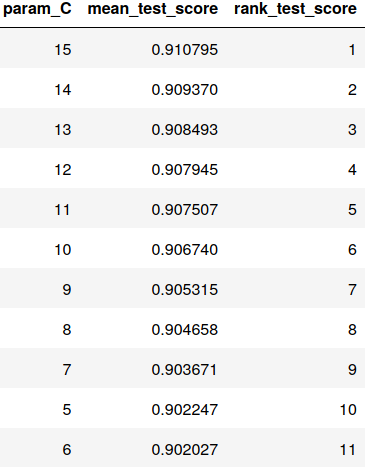
\includegraphics[width=50mm]{imgs/tune-svm2}
  }
  \subfigure[Acabamos eligiendo $C=65$.]{
    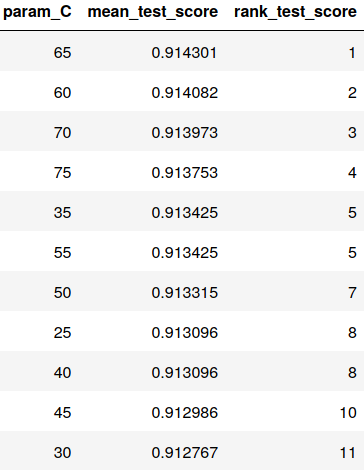
\includegraphics[width=50mm]{imgs/tune-svm3}
  }
  \caption{Búsquedas en cuadrícula de la configuración de SVM con CV.}
  \label{fig:tune-svm}
\end{figure}

Esta configuración consigueen el intento 6 nuestra mejor puntuación
hasta el momento. Pero tras descubrir que la validación cruzada es
propensa a sobreajustar, realizamos una segunda búsqueda para el
parámetro $C$ y elegimos $C=40$.

\begin{figure}[H]
  \centering
  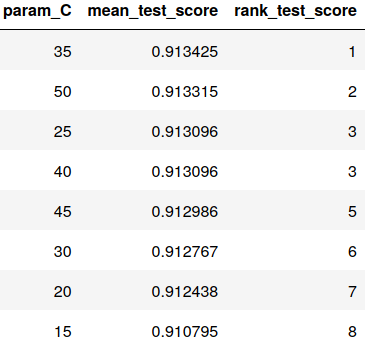
\includegraphics[width=50mm]{imgs/val-svm}
  \caption{Búsqueda en cuadrícula de la configuración de SVM con el conjunto de validación.}
  \label{fig:val-svm}
\end{figure}

Con esta configuración, consigue mejorar su score en el intento 27,
pero queda lejos de otros modelos como GradientBoosting.

\subsection{KNN}

Sólo hemos probado un intento con este modelo, el 5, y los resultados
han sido bastante malos tanto en CV como en test. Los parámetros que
hemos ajustado son la métrica (euclídea, Manhattan o máximo), el
número de vecinos y los pesos (uniformes o inversamente proporcionales
a la distancia). En la Figura \ref{fig:tune-knn} vemos la última
búsqueda en cuadrícula para este modelo y la configuración definitiva
con la que realizamos el intento.

\subsection{Boosting}

Boosting ha sido la técnica más efectiva entre las que he probado. Es
por ello que probamos diferentes variantes e implementaciones. Al
contrario que en el resto de modelos, algunas de las implementaciones
(\href{https://lightgbm.readthedocs.io/en/latest/pythonapi/lightgbm.LGBMClassifier.html}{Lightgbm}
y
\href{https://xgboost.readthedocs.io/en/latest/python/python_api.html#xgboost.XGBClassifier}{XGBoost})
no son de \textit{sklearn}.

El primer algoritmo que intentamos es GradientBoosting, ajustamos el
learning rate (obtenemos 0.1) y el número de estimadores (obtenemos
500) y superamos en el intento 8 el mejor score que habíamos obtenido
hasta el momento. El éxito de este modelo nos lleva a considerar otras
implementaciones de esta técnica.

Configuramos varios parámetros (número de estimadores, learning rate y
profundidad máxima de los estimadores) de AdaBoost (que utiliza una
función de perdida exponencial) para el intento 10, pero conseguimos
resultados bastante peores, quizá debido al sobreajuste.

Probamos una configuración más compleja de GradientBoosting para el
intento 13, añadiendo a la cuadrícula los parámetos subsample
(proporción de la muestra con la que entrena cada estimador simple) y
profundidad máxima de los estimadores simples. Pero empeoramos los
resultados sobre test. Igual ocurre en el intento 21, donde utilizamos
el conjunto de validación para ajustar los parámetos.

También probamos diversas configuraciones de LightGBM, una variante de
GradientBoost mucho más rápida, usamos validación cruzada (intentos 23
y 24) y validación simple (intento 22) para ajustar los
parámetos. Pero no conseguimos que este modelo iguale el desempeño de
GradientBoosting. También probamos la implementación de
\textit{sklearn} de esta técnica, HistGradBoost, con configuraciones
obtenidas por ambos sistemas de validación (intentos 29, valicación; y
30, CV). Igualmente, este modelo se queda por debajo. Ajustamos el
learning rate y el número de estimadores, así como la profundidad
máxima y el número máximo de nodos hoja de los mismos.

Finalmente, configurando XGBoost con el conjunto de validación,
obtenemos un resultado a la altura de GradientBoosting (intento 28).

\begin{figure}[H]
  \centering
  \subfigure[Configuración de HistGradientBoosting para el intento 29.]{
    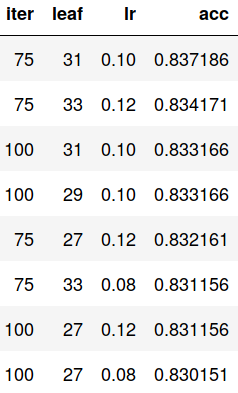
\includegraphics[width=45mm]{imgs/val-hist}
  }
  \subfigure[Configuración de LightGBM para el intento 22.]{
    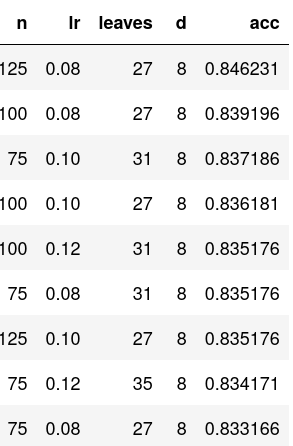
\includegraphics[width=55mm]{imgs/tune-lgbm22}
  }
  
  \subfigure[Configuración de LightGBM para el intento 23.]{
    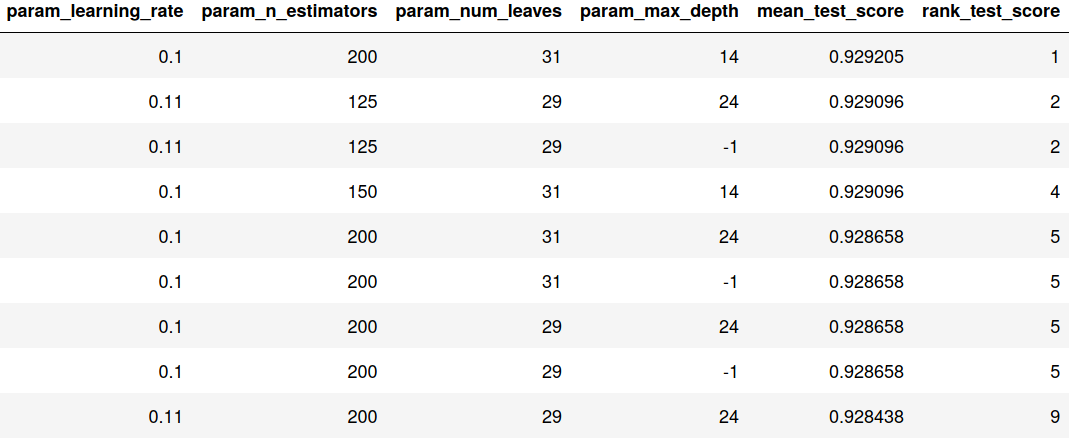
\includegraphics[width=140mm]{imgs/tune-lgbm23}
  }
  \caption{Búsquedas en cuadrícula para configurar distintos algoritmos de boosting.}
  \label{fig:tune-svm}
\end{figure}

\subsection{Stacking}

Stacking es una técnica que combina distintos clasificadores para
mejorar el desempeño que tienen por separado, necesitamos varios
clasificadores que ya presenten un desempeño decente. Stacking se ve
mejorada cuanto mayor sea el número de clasificadores, su calidad y su
variedad. Por lo que tenemos que encontrar un compromiso entre
cantidad, calidad y variedad de los estimadores para sacarle el máximo
partido.

Este modelo entrena los estimadores que apila a la vez que un
estimador final (Regresión Logística) sobre los resultados, y utiliza
validación cruzada para evaluar a qué estimadores debe de darles más
peso. Su ejecución es muy lenta, por lo que en algunos experimentos
omitimos la validación cruzada.

Nuestro primer intento de stacking es el 9, que combina el Random
Forest por defecto, el MLP con la configuración del intento 4, el SVM
con la configuración del intento 6 y el GradientBoosting del intento
8. No consigue superar al GradientBoosting, por lo que alguno o varios
del resto de estimadores está minando su eficacia.

Probamos en el intento 16 distintos (cuatro) GradientBoosting con
número de estimadores y learning rates diferentes, y fijamos nuestro
récord personal. En el siguiente intento permitimos
(\texttt{passthrough=True}) que el clasificador final también aprenda
sobre la muestra además de sobre los resultados, pero empeoreamos
ligeramente el desempeño.

En los intentos 19 y 20 añadimos algunos HistGradientBoosting con
diferentes configuracioens, pero también empeoramos el desempeño.

Finalmente en el intento 31, ya tenemos una batería más amplia y
variada de modelos con calidad decente. Probamos Stacking con tres
algoritmos basados en Boosting (GradientBoosting del intento 8,
XGBoost del 28 y HistGradientBoosting del 29) y el nuevo MLP (intento
26). Conseguimos mejorar la mejor puntuación hasta el momento.

Eliminando el que peor desempeño tenía, HistGradientBoosting,
conseguimos en el intento 32 nuestra puntuación definitiva. Finalmente,
comprobamos en el intento 33 que eliminar el segundo con peor
desempeño (MLP) empeora los resultados.

\pagebreak

\section{Otras pruebas fallidas}

Describo otras estrategias que he intentado pero desechado por obtener
scores bastante bajos en validación.

\subsection{Experimentos con la columna descuento} \label{descuento}

Al no tener en cuenta el descuento, es lógico pensar que los coches
con valores altos en este campo pueden confundir a los algoritmos, ya
que podrían estar en una categoría más baja de la que realmente
estarían si no tuviesen descuento. Del mismo modo, es posible que
fracasemos al clasificar datos de test porque un elevado descuento los
sitúe en una categoría más baja que la que le correspondería.

Pruebo dos ideas en esta línea. La primera en el intento 3, en la que
elimino los ejemplos de train que presentan algún descuento. Esto
evita que los algoritmos sean entrenados erróneamente, pero sigue
existiendo el problema en el test. No logro ninguna mejora con esta
idea. Además, estoy suponiendo que las instancias con valor NA en
descuento se trata de coches sin descuento, lo cual podría no ocurrir.

Bajo esta suposición pruebo una segunda idea en esta línea, que
corresponde al intento 14. Sustituyo por 0 los valores perdidos en la
columna Descuento en lugar de eliminar la columna, tanto en train como
en test. Tampoco logro ninguna mejora con esta idea.

Finalmente, desecho cualquier esperanza de obtener información con el
siguiente experimento: Primero separo del conjunto de train un
conjunto de validación correspondiente a todos los ejemplos que
cuentan con el campo descuento. Entreno mi mejor algoritmo hasta el
momento (GradientBoosting con 500 estimadores) con los datos restantes
y realizo predicción sobre el conjunto de validación. Obtengo las
siguiente tablas:

\begin{figure}[H]
  \centering \subfigure[Fallos y aciertos en las predicciones.]{
    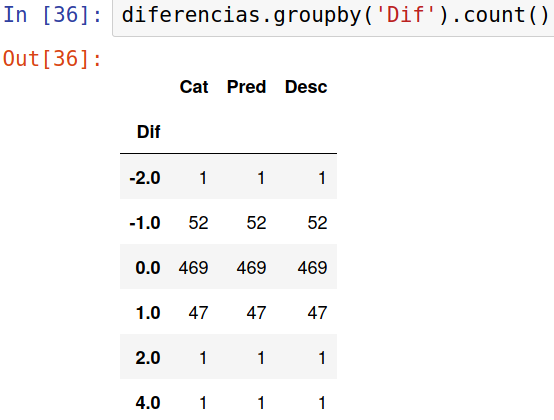
\includegraphics[width=85mm]{imgs/descuento-count} }
  \subfigure[Descuentos en las predicciones acertadas y falladas.]{
    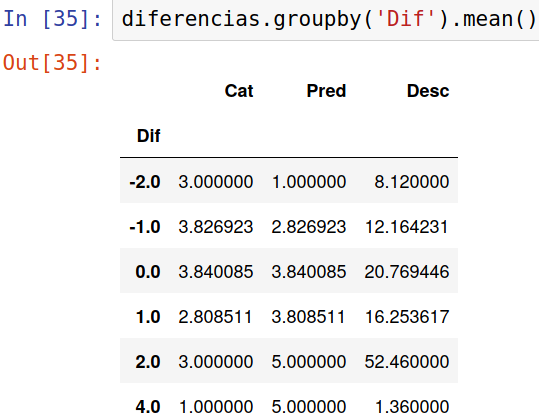
\includegraphics[width=85mm]{imgs/descuento-mean} }
  \caption{Relación entre los descuentos y la exactitud de las predicciones.}
  \label{fig:descuento}
\end{figure}

En la tabla de la izquierda, observamos que los fallos se producen
aproximadamente en la misma medida por exceso ($\text{Dif}>0$,
predecimos una clase más cara a la correspondiente) que por defecto
($\text{Dif}<0$, predecimos una clase más barata a la
correspondiente). En la tabla de la derecha observamos que los valores
de descuento no son mayores en las instancias que fallamos, sino en
las que acertamos. Tampoco hay una diferencia significativa entre el
descuento medio de las instancias que fallamos por exceso o
defecto. Por tanto, no parece que altos descuentos lleven a mayor
error en las predicciones.

\pagebreak

\subsection{Naive-Bayes}

El modelo Naive-Bayes requiere un preprocesado algo distinto, ya que
asume independencia en las variables y la binarización de variables
categóricas impide esta propiedad. Intentamos combinar el preprocesado
2 con PCA para quedarnos con menos variables y además
incorreladas. Probando distintos valores para la proporción de
variabilidad explicada, no logramos pasar de accuracy 0.6 en
validación cruzada, por lo que no aplicamos este modelo a ningún
intento.

\subsection{Clustering}

La validación (y validación cruzada) acostumbra a obtener una
estimación pesimista del desempeño de los modelos, debido a que
entrenan con menos datos. Claramente, en este caso no la tenemos. En
el caso de validación cruzada es lógico pensar que el problema es el
que comentamos en la Sección \ref{val-sobreajuste} con el
oversampling, pero en validación simple no se da este problema, así
que podría ocurrir que existiese cierto sesgo entre los datos de test
y de entrenamiento, normalmente este problema limita nuestras
posibilidades y no tiene solución.

En un intento, quizá desesperado, de atajar este problema. Probamos
técnicas de aprendizaje no supervisado. Utilizamos un preprocesado
como el 3 (binarización de características nominales y reescalado de
las variables) pero sin balanceo de clases. Mezclamos los datos de
train y test, y aplicamos K-means y Ward con $K=5$ con la esperanza de
que el tamaño de los clusters concuerde con las instancias de train
que deberían pertenecer a esos clusters (para que sea factible que se
hubiese formado un cluster por clase), pero no logramos nada.

\begin{figure}[H]
  \centering 
  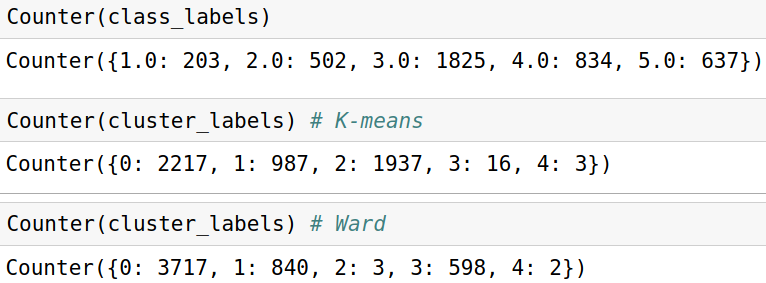
\includegraphics[width=110mm]{imgs/cluster1}
  \caption{Tamaño de los clusters comparado con el número de
    instancias de train en cada clase.}
  \label{fig:cluster1}
\end{figure} \vspace{-3mm}

Como observamos, los clusters 4 de las segmentaciones no puede
contener a ninguna clase.

Probamos a introducir cinco nuevas dimensiones, a los datos de test
les ponemos el 0 en todas, mientras que a los datos de entrenamiento
les asignamos un valor $r>0$ en una (relativa a su clase) lo
suficientemente grande para forzar que los datos de la misma clase
acaben en el mismo cluster. Los datos de test no tendrían
predisposición a formar parte de ningún cluster respecto a estas cinco
dimensiones. Por tanto, quizá las instancias de test se vean
``arrastradas'' al cluster correspondiente a su clase según sus
valores en el resto de variables (las originales). 

\begin{figure}[H]
  \centering 
  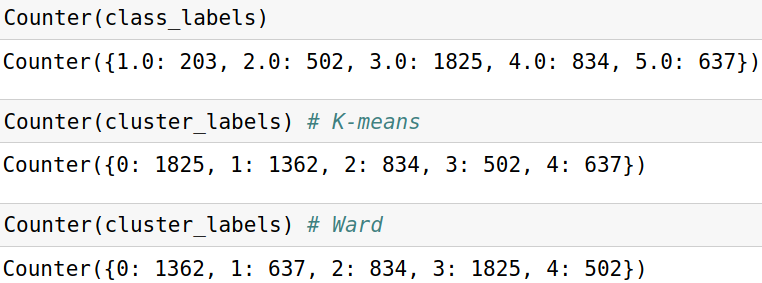
\includegraphics[width=110mm]{imgs/cluster2}
  \caption{Tamaño de los clusters comparado con el número de
    instancias de train en cada clase, forzando a que cada clase esté contenida en un cluster.}
  \label{fig:cluster2}
\end{figure} \vspace{-3mm}

Como observamos, las instancias de test se ven arrastradas todas al
mismo cluster, el cluster 1 de K-means y el 0 de Ward. Luego no hemos
obtenido ninguna información.

\section{Webgrafía}

Algoritmos de \textit{sklearn}:
\begin{itemize}

\item Random Forest: \href{https://scikit-learn.org/stable/modules/generated/sklearn.ensemble.RandomForestClassifier.html}{https://scikit-learn.org/stable/modules/generated\\/sklearn.ensemble.RandomForestClassifier.html}
\item SVM: \href{https://scikit-learn.org/stable/modules/generated/sklearn.svm.SVC.html}{https://scikit-learn.org/stable/modules/generated/sklearn.svm.SVC.html}
\item Gaussian Naive-Bayes: \href{https://scikit-learn.org/stable/modules/generated/sklearn.naive_bayes.GaussianNB.html}{https://scikit-learn.org/stable/modules/generated\\/sklearn.naive\_bayes.GaussianNB.html}
\item KNN \href{https://scikit-learn.org/stable/modules/generated/sklearn.neighbors.KNeighborsClassifier.html}{https://scikit-learn.org/stable/modules/generated/sklearn.neighbors.KNeighborsClassifier.html}
\item MLP: \href{https://scikit-learn.org/stable/modules/generated/sklearn.neural_network.MLPClassifier.html}{https://scikit-learn.org/stable/modules/generated/sklearn.neural\_network.MLPClassifier.html}
\item GradientBoosting: \href{https://scikit-learn.org/stable/modules/generated/sklearn.ensemble.GradientBoostingClassifier.html}{https://scikit-learn.org/stable/modules/generated/sklearn.ensemble.GradientBoostingClassifier.html}
\item HistGradientBoosting: \href{https://scikit-learn.org/stable/modules/generated/sklearn.ensemble.HistGradientBoostingClassifier.html}{https://scikit-learn.org/stable/modules/generated\\/sklearn.ensemble.HistGradientBoostingClassifier.html}
\item Stacking: \href{https://scikit-learn.org/stable/modules/generated/sklearn.ensemble.StackingClassifier.html}{https://scikit-learn.org/stable/modules/generated/sklearn.ensemble.StackingClassifier.html}
\item K-means: \href{https://scikit-learn.org/stable/modules/generated/sklearn.cluster.KMeans.html}{https://scikit-learn.org/stable/modules/generated/sklearn.cluster.KMeans.html}
\item Clustering aglomerativo (Ward):
  \href{https://scikit-learn.org/stable/modules/generated/sklearn.cluster.AgglomerativeClustering.html}{https://scikit-learn.org/stable/modules/generated/\\sklearn.cluster.AgglomerativeClustering.html}
\end{itemize}

Otros algoritmos:
\begin{itemize}
\item LightGBM: \href{https://lightgbm.readthedocs.io/en/latest/pythonapi/lightgbm.LGBMClassifier.html}{https://lightgbm.readthedocs.io/en/latest/pythonapi/lightgbm.LGBMClassifier.html}
\item XGBoost: \href{https://xgboost.readthedocs.io/en/latest/python/python_api.html#xgboost.XGBClassifier}{https://xgboost.readthedocs.io/en/latest/python/python\_api.html\#xgboost.XGBClassifier}
\end{itemize}
\end{document}
